\chapter{Einführung}\label{AppendixEinführung}

\section{Installationsanleitung}

\subsection{Benötigte Software}

\subsubsection{Server}
- geoip db
- imagemagick

\subsubsection{Testumgebung}
- webdriver (npm, für tests)

\subsection{Umgebungsvariablen}

\begin{longtable}[]{@{}ll@{}}
  \toprule
  \textbf{Name}            & \textbf{Beschreibung}\tabularnewline
  \midrule
  AWS\_S3\_BUCKET          & \tabularnewline
  AWS\_ACCESS\_KEY\_ID     & \tabularnewline
  AWS\_SECRET\_ACCESS\_KEY & \tabularnewline
  AWS\_REGION              & \tabularnewline
  AWS\_S3\_SCHEME          & \tabularnewline
  AWS\_S3\_HOST            & \tabularnewline
  AWS\_S3\_PORT            & \tabularnewline
  GIGPILLAR\_ASSET\_HOST   & \tabularnewline
  POSTGRES\_USER           & \tabularnewline
  POSTGRES\_PASSWORD       & \tabularnewline
  POSTGRES\_DB             & \tabularnewline
  POSTGRES\_HOSTNAME       & \tabularnewline
  POSTGRES\_POOL\_SIZE     & \tabularnewline
  GEOIP\_DATABASE\_FILE    & \tabularnewline
  \bottomrule
\end{longtable}

\clearpage
\subsection{Initialen Benutzer erstellen}

Es wurde ein Skript erstellt um den ersten, initialen Benutzer zu erstellen.
Dies sollte vorallem für Testzwecke verwendet werden und nicht auf der
produktiven Umgebung.

\begin{lstlisting}[language=bash,frame=single]
$ mix gigpillar.create_user
\end{lstlisting}

\noindent{}Beispiel einer erfolgreichen Durchführung des Skripts:

\begin{figure}[!htb]
  \centering
  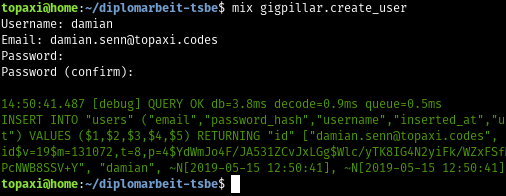
\includegraphics[width=0.9\textwidth]{einfuehrung/create-user.png}
  \caption{Initialen Benutzer erstellen}
\end{figure}
